%\documentclass{beamer}
\documentclass[handout]{beamer}
\mode<presentation> {%
	\usetheme[]{Boadilla}
	\usecolortheme{orchid}
	\setbeamercovered{transparent}
	\setbeamersize{text margin left=0.7cm}
  \setbeamersize{text margin right=0.7cm}
  \setbeamertemplate{enumerate item}[square]
  \setbeamertemplate{enumerate subitem}[circle]
  \setbeamertemplate{enumerate subsubitem}[>]
  \setbeamertemplate{itemize item}[square]
  \setbeamertemplate{itemize subitem}[circle]
  \setbeamertemplate{itemize subsubitem}[>]
}

\usepackage{hyperref}
% \usepackage{bm} % Tipo de letra
\usepackage[utf8]{inputenc}
\usepackage[spanish]{babel}
% \usepackage{times}
\usepackage[T1]{fontenc}
\usepackage{graphicx}
\usepackage{multirow}
\usepackage{xcolor}
\usepackage{colortbl}
\usepackage{tikz}
\usetikzlibrary{positioning}
\usetikzlibrary{shapes.multipart,decorations.pathreplacing}
\tikzstyle{bloque}=[rectangle,rounded corners=2pt,draw=black!60,fill=black!5,very thick,minimum size=5mm,align=center]%
\tikzstyle{arrow}=[very thick,color=black!60]%

\definecolor{olivegreen}{rgb}{0.0,0.5,0.0}

\title[Procesamiento de Señales]{Introducción: Sistemas LTI}
\author[Jesús Chacón Sombría]{%
\textit{Ingeniería Electrónica de Comunicaciones }\\
\vspace{0.6cm}
\small Jesús Chacón Sombría \\
\small María José Gómez Silva}

\institute[DACYA. UCM] {%\inst{1}%
	\footnotesize  Departamento de Arquitectura de Computadores y Automática\\
  Universidad Complutense de Madrid
}

\date[Descripción General ] % (optional)
{\footnotesize Curso 2022-2023 }%{\today / Master}
\subject{Talks}

\pgfdeclareimage[height=1cm]{logo}{../ucm.png}

\usepackage[absolute,overlay]{textpos}
\setlength{\TPHorizModule}{1mm}
\setlength{\TPVertModule}{1mm}
\newcommand{\MyLogo}{%
\begin{textblock}{14}(116.0,0.6)
  \pgfuseimage{logo}
\end{textblock}
}

\makeatletter
\numberwithin{section}{part}
\AtBeginPart{
\beamer@tocsectionnumber=0\relax
\frame{\partpage}
}
\makeatother

\begin{document}

\begin{frame}
  \titlepage
\end{frame}

\newcommand*\oldmacro{}%
\let\oldmacro\insertshorttitle%
\renewcommand*\insertshorttitle{%
	\MyLogo
\oldmacro\hfill%
}

\AtBeginSection[]
{
  \begin{frame}%<beamer>
    \frametitle{Esquema}
  \small
    \tableofcontents[sectionstyle=show/shaded,subsectionstyle=show/shaded/hide]
  \end{frame}
}

\AtBeginSubsection[]
{
  \begin{frame}%<beamer>
    \frametitle{Esquema}
  \small
   \tableofcontents[sectionstyle=show/shaded,subsectionstyle=show/shaded/hide]
      \end{frame}
}

\section{Sistemas}
\subsection{Tipos de Sistemas}

\begin{frame}
  \frametitle{Tipos de Sistemas I}

  \vspace{-0,3cm}

  \begin{figure}
    \centering
    \small
    \begin{tikzpicture}
      \node[bloque,minimum width=15mm] (T) {T};
      \node (x) [left=of T] {};
      \node (y) [right=of T] {};
      \draw[arrow,->] (x.east) -- (T.west) node [midway,above] {$x(\cdot)$};
      \draw[arrow,->] (T.east) -- (y.west) node [midway,above] {$y(\cdot)$};
    \end{tikzpicture}
  \end{figure}
  \vspace{-0,25cm}
  \begin{itemize}
    \item <1-> Seg\'{u}n el n\'{u}mero de variables de entrada y de salida:
    \begin{itemize}
      \item \color{olivegreen}{SISO }\color{black}  (Single-Input, Single-Output): 1 variable de entrada, 1 variable de salida
      \item \alert{MIMO} (Multiple-Input, Multiple-Output): multiples variables de entrada, multiples variables de salida
      \item \alert{SIMO} (Single-Input, Multiple-Output): 1 variable de entrada, multiples variables de salida
      \item \alert{MISO} (Multiple-Input, Single-Output): multiples variables de entrada, 1 variable de salida
      \item \alert{Aut\'{o}nomo}:  sistema sin entradas de control
    \end{itemize}

    \item <2-> Según las características de la variable independiente:
    \begin{itemize}
      \item \alert{Sistemas Continuos}: admite/devuelve señales continuas
      \item \alert{Sistemas Discretos}: admite/devuelve señales discretas
      \item \alert{Conversores}: Admiten señales continuas/discretas y devuelven señales discretas/continuas
    \end{itemize}
  \end{itemize}

  \vspace{-0.4cm}

\end{frame}

%%%%%%%%%%%%%%%%%%%%%%%%%%%%%%%%%%%%%%%%%%%%

\begin{frame}
  \frametitle{Tipos de Sistemas II}

  \vspace{-0,3cm}

  \begin{figure}
    \centering
    \small
    \begin{tikzpicture}
      \node[bloque,minimum width=15mm] (T) {T};
      \node (x) [left=of T] {};
      \node (y) [right=of T] {};
      \draw[arrow,->] (x.east) -- (T.west) node [midway,above] {$x(\cdot)$};
      \draw[arrow,->] (T.east) -- (y.west) node [midway,above] {$y(\cdot)$};
    \end{tikzpicture}
  \end{figure}

  \vspace{-0.25cm}

  \begin{itemize}
    \item <1-> Seg\'{u}n la existencia o no de procesos aleatorios:
    \begin{itemize}
      \item \alert{Sistemas Deterministas}: no hay procesos aleatorios involucrados, por lo que la respuesta del sistema ante la mismas entradas es siempre la misma.
      \item \alert{Sistemas Estoc\'{a}sticos}: hay procesos aleatorios involucrados, por lo que la respuesta del sistema ante la mismas entradas depende del experimento.
    \end{itemize}

    \item <2-> Causales/no causales:
    \begin{itemize}
      \item \color{olivegreen}{Sistemas Causales}\color{black}: La salida del sistema en un instante únicamente depende de las entradas hasta dicho instante de tiempo. 

  \vspace{0.2cm}

     \hspace{0.4cm} $y(t)=\bm{T} [ \:x(\tau)|\tau<=t\: ] \: \:$       ó          $\: \:y[n]=\bm{T}[\: x[k]|k<=n\:]$ 
     
     \vspace{0.2cm}
     
      \item \alert{Sistemas No Causales}: La salida del sistema en un instante depende de la entrada en instantes posteriores. No es físicamente realizable. 
    \end{itemize}

  \end{itemize}

\vspace{-0.4cm}

\end{frame}

% %%%%%%%%%%%%%%%%%%%%%%%

\begin{frame}
\frametitle{Tipos de Sistemas III}

\vspace{-0,1cm}

\begin{figure}
  \centering
  \small
  \begin{tikzpicture}
    \node[bloque,minimum width=15mm] (T) {T};
    \node (x) [left=of T] {};
    \node (y) [right=of T] {};
    \draw[arrow,->] (x.east) -- (T.west) node [midway,above] {$x(\cdot)$};
    \draw[arrow,->] (T.east) -- (y.west) node [midway,above] {$y(\cdot)$};
  \end{tikzpicture}
  \end{figure}

  \vspace{-0.25cm}
  \begin{itemize}
    \item <1-> Respecto a la memoria del sistema:
    \begin{itemize}
      \item \alert{Sistemas Estáticos}: La salida del sistema en un instante depende únicamente de la entrada en dicho instante. 
  
      \vspace{0.1cm}
      \hspace{1cm}    $y(t)=\bm{T}[\:x(t)\:] \: \:$       ó          $\: \:y(n)=\bm{T}[\:x[n]\:]$ 
  
      \vspace{0.1cm}    
      \item \color{olivegreen}{Sistemas Dinámicos}\color{black}: La salida del sistema en un instante depende de la historia pasada del sistema. Los sistemas dinámicos continuos se pueden modelar con una ecuación diferencial. Los discretos con una ecuación en diferencias.

      \vspace{0.1cm}

      $y(t)=\bm{T}[\:x(\tau) | \tau \subseteq \mathbb{R} \le t\:] \: \:$       ó          $\: \:y(n)=\bm{T}[\:x[k] | k \subseteq \mathbb{Z} \le n\:]$
      \vspace{0.1cm}
 
    \end{itemize}

    \item <2-> Estable/inestable:
    \begin{itemize}
      \item \color{olivegreen}{Sistemas Estables}\color{black}: cuando responde con una salida acotada en amplitud ante cualquier entrada acotada (BIBO-estable: bounded-input, bounded-output). 

      \vspace{0.1cm}

      \hspace{1.8cm} $|x(\cdot)|< B_1  \rightarrow  |y(\cdot)|< B_2$  
     
      \vspace{0.1cm}
      \item \alert{Sistemas Inestables}\color{black}: cuando no cumplen la propiedad anterior. 


    \end{itemize}

%\item <1-> Invertibles/no invertibles:
%\begin{itemize}
%\item \alert{Sistemas Invertibles}\color{black}: en los que  existe una función $\bm{T}^{-1}[\cdot]$ que permite recuperar la entrada a partir de la salida. 

%  \vspace{0.1cm}

%     \hspace{1.8cm} $x(\cdot)=\bm{T}^{-1} [\: \bm{T}[\:x(\cdot)\: ]  \: ]$  
     
% \vspace{0.1cm}
     

     
%\item \alert{Sistemas No Invertibles}: en los que no existe la función $\bm{T}^{-1}[\cdot]$.
%\end{itemize}
  \end{itemize}
\end{frame}

% %%%%%%%%%%%%%%%%%




\begin{frame}
  \frametitle{Tipos de Sistemas IV}

  \vspace{-0.4cm}

  \begin{columns}[c]
    \hspace{-1.8cm}\begin{column}{12cm}
      \small 
      \begin{itemize}
        \item <1-> Sistemas lineales/no lineales:
        \begin{itemize}
          \item \color{olivegreen}{Sistemas Lineales}\color{black}: Los que cumplen el principio de superposición, i.e. la respuesta del sistema producido por varias fuentes excitadoras a la vez es la suma de las respuestas producidas por las fuentes individualmente.
          \vspace{0.1cm}
          $\bm{T}[\:\alpha x_1(\cdot)+\beta x_2(\cdot)\:]=\alpha \bm{T}[\:x_1(\cdot)\:] + \beta \bm{T}[\: x_2(\cdot) \:] =\alpha y_1(\cdot)+ \beta y_2(\cdot)$
          \vspace{0.1cm}
          \item \alert{Sistemas No Lineales}: Los que no cumplen el principio de superposición. Los sistemas reales son sistemas no lineales, aunque pueden ser tratados como sistemas lineales en torno a un determinado punto de operaci\'{o}n.
        \end{itemize}
      \end{itemize}
    \end{column}
    \hspace{-7cm}\begin{column}{4cm}
      \vspace{-3.75cm}
      \small
      \begin{tikzpicture}
        \node[bloque,minimum width=15mm] (T) {T};
        \node (x) [left=of T] {$x(\cdot)$};
        \node (y) [right=of T] {$y(\cdot)$};
        \draw[arrow,->] (x.east) -- (T.west);
        \draw[arrow,->] (T.east) -- (y.west);
      \end{tikzpicture}
    \end{column}
  \end{columns}
  \vspace{0.2cm}
  \begin{columns}[c]
    \begin{column}{4cm}
      \includegraphics[width=3.8cm]{./Figuras/FigLT1.eps} 
    \end{column}
    \begin{column}{4cm}
      \includegraphics[width=3.8cm]{./Figuras/FigLT2.eps} 
    \end{column}
    \begin{column}{4cm}
      \includegraphics[width=3.8cm]{./Figuras/FigLT3.eps} 
    \end{column}
  \end{columns}
\end{frame}

%%%%%%%%%%%%%%%%%%%%%%%%%%%%%%%%

\begin{frame}
  \frametitle{Tipos de Sistemas V}
  \small
  \vspace{-0.4cm}

  \begin{columns}[c]
    \hspace{-0.2cm}\begin{column}{12cm}
      \begin{itemize}
        \item <1-> Sistemas temporalmente invariantes/no invariantes:
        \vspace{-0.2cm}
        \begin{itemize}
          \item \color{olivegreen}{Sistemas Temporalmente  Invariantes}\color{black}: Aquellos en los que su relación entrada-salida es invariante en el tiempo (a una entrada desplazada temporalmente le corresponde la misma salida desplazada el mismo valor).
          \vspace{0.1cm}
          $\bm{T}[\: x(t)\:]=y(t) \rightarrow \bm{T}[\: x(t-t_0)\:]=y(t-t_0)$
          \vspace{0.1cm}
          $\bm{T}[\: x[n]\:]=y(n) \rightarrow \bm{T}[\: x(n-N_0)\:]=y(n-N_0)$
          \vspace{0.1cm}
          \item \alert{Sistemas Temporalmente No  Invariantes}: Los que no cumplen la propiedad anterior.
      \end{itemize}

      \begin{columns}[c]
        \begin{column}{4cm}
          \includegraphics[width=4cm]{./Figuras/FigLT1B.eps} 
        \end{column}
        \begin{column}{4cm}
          \includegraphics[width=4cm]{./Figuras/FigLT2B.eps} 
        \end{column}
      \end{columns}

      \vspace{-0.2cm}
      \item \color{olivegreen}{Sistemas Lineales Temporalmente Invariantes}: Sistemas LTI
      \end{itemize}
    \end{column}
    \hspace{-3.0cm}\begin{column}{4cm}
      \vspace{7.25cm}
      \small
      \begin{tikzpicture}[scale=0.8,every node/.style={scale=0.8}]
        \node[bloque,minimum width=15mm] (T) {T};
        \node (x) [left=of T] {};
        \node (y) [right=of T] {};
        \draw[arrow,->] (x.east) -- (T.west) node [midway,above] {$x(\cdot)$};
        \draw[arrow,->] (T.east) -- (y.west) node [midway,above] {$y(\cdot)$};
      \end{tikzpicture}
    \end{column}
  \end{columns}

\end{frame}
\subsection{Sistemas LTI}

\begin{frame}
\frametitle{Sistemas LTI}

\vspace{-0,3cm}

  \begin{figure}
    \centering
    \small
    \begin{tikzpicture}
      \node[bloque,minimum width=15mm] (T) {LTI};
      \node (x) [left=of T] {};
      \node (y) [right=of T] {};
      \draw[arrow,->] (x.east) -- (T.west) node [midway,above] {$x(\cdot)$};
      \draw[arrow,->] (T.east) -- (y.west) node [midway,above] {$y(\cdot)$};
    \end{tikzpicture}
  \end{figure}

  \begin{itemize}
    \item <1-> Constituyen una clase de sistemas muy importantes en procesamiento de señales, control de sistemas, teoría de la comunicación.

    \item Características más relevantes:

    \begin{itemize}

      \item <1-> La respuesta de un sistema LTI a una entrada puede obtenerse como la \alert{convolución} de la entrada con la respuesta del sistema a la entrada impulso unitario.

      \item <1-> Las \alert{transformadas} de Laplace, Z, Fourier \alert{de la convolución es el producto de las transformadas}. 

      \item Por lo tanto, podemos calcular la respuesta de los sistemas LTI ante una entrada a partir del producto de la transformada de la entrada y de la transformada del sistema. 

    \end{itemize}

  \end{itemize}

  \vspace{-0.4cm}

\end{frame}

%%%%%%%%%%%%%%%%%%%%%%%%%%%%%%%%%%%%%%%%%%%%


\begin{frame}
\frametitle{Respuesta temporal sistema LTI}

\vspace{-0,3cm}


\begin{itemize}
\item <1-> \alert{Sistemas Continuos}:

\begin{itemize}
\item Respuesta al impulso (función ponderatriz):   $\bm{T}[\delta(t)]=h(t)$
	
	\vspace{0,1cm}
	
\item Respuesta a una entrada arbitraria:

\vspace{0,2cm}

\footnotesize $\begin{array}{ll}\color{red}\!\!\bm{T}[x(t)]\color{black}\!\!\!\!\!\!&=\bm{T}[(x\!*\!\delta)(t)]\!=\!\bm{T}[\int_{-\infty}^{\infty} \! x(\tau)\delta({t\!-\!\tau})d\tau] \!=\!\int_{-\infty}^{\infty}\bm{T}[x(\tau)\delta({t\!-\!\tau})]d\tau \!=\\ [0.2cm]  & =\int_{-\infty}^{\infty} x(\tau) \bm{T}[\delta({t\!-\!\tau})]d\tau  =\int_{-\infty}^{\infty} x(\tau)  h(t\!-\!\tau) d\tau \color{red}= (x*h)(t)\color{black} \end{array}$


\end{itemize}


\item <2-> \alert{Sistemas Discretos}:

\begin{itemize}
\item Respuesta al impulso (función ponderatriz):   $\bm{T}[\delta(n)]=h(n)$
	
	\vspace{0,1cm}
	
\item  Respuesta a una entrada arbitraria:

\vspace{0,1cm}

\footnotesize $\begin{array}{ll}\color{red}\!\!\bm{T}[x(n)]\color{black}\!\!\!\!\!\!&=\!\bm{T}[(x\!*\!\delta)(n)]\!=\!\bm{T}[\sum_{k=-\infty}^{\infty} \! x(k)\delta({n\!-\!k})] \!=\!\!\sum_{k=-\infty}^{\infty}\! \!\bm{T}[x(k)\delta({n\!-\!k})]\!=\\ [0.2cm]  & =\!\sum_{k=-\infty}^{\infty} x(k) \bm{T}[\delta({n\!-\!k})]  \!=\!\sum_{k=-\infty}^{\infty} x(k)  h(n\!-\!k) \color{red} \!=\! (x\!*\!h)(n)\color{black} \end{array}$

\vspace{0,2cm}
\end{itemize}


\item <3-> \small La respuesta de un  sistema LTI a cualquier entrada $x(\cdot)$ se puede calcular como la convolución de la entrada y la respuesta del sistema a la entrada impulso $h(\cdot)$.

\vspace{0,1cm}

\hspace{2cm} \alert{$h(\cdot)=\bm{T}[\delta(\cdot)]  \rightarrow  \bm{T}[x(\cdot)]=(x* h)(\cdot)$}


\end{itemize}


\end{frame}

%%%%%%%%%%%%%%%%%%%%%%%%%%%%%%%%%%%%%%%%%%%%


\begin{frame}
\frametitle{Sistemas LTI continuos I}

\vspace{-0,3cm}


\begin{itemize}
\item <1-> \alert{Transformada de Laplace (TL)}:

\begin{itemize}
\item Bilateral:    $\mathcal{L}{[x(t)]}\!=\!X(s)\!=\! \int_{-\infty}^{\infty} \! \!x(t) e^{-t s} dt \:$ con   $s \in \mathbb{C}$


\vspace{0.1cm}

\item \color{olivegreen} Unilateral:    $\mathcal{L}{[x(t)]}\!=\!X(s)\!= \!\int_{0}^{\infty} \! \! x(t) e^{-t s}dt  \:$ con   $s \in \mathbb{C}$, $x(t)$ causal \color{black}

\vspace{-0.4cm}

\end{itemize}

\item <2-> \alert{Propiedades} (similares, se diferencian en las condiciones iniciales que aparecen en las derivadas):

\begin{itemize}
\item Linealidad : $\mathcal{L}[\alpha x_1(t)+\beta  x_2(t)]=\alpha \mathcal{L}[x_1(t)]+\beta \mathcal{L}[x_2(t)]$
\vspace{0.2cm}
\item Desplazamiento temporal: $\mathcal{L}[x(t-t_0)]=e^{-st_0} \mathcal{L}[x(t)]$
\vspace{0.2cm}
\item Derivada: $\mathcal{L}[\frac {dx(t)}{dt}]=s \mathcal{L}[x(t)]\color{olivegreen}-x(0)\color{black}$
\vspace{0.2cm}
\item Convolución: $\mathcal{L}[{(x*y)(t)}]= \mathcal{L}[x(t)]\mathcal{L}[y(t)]$
\end{itemize}

\item <3-> \alert{TL de la respuesta del sistema}:

\vspace{0.2cm}

\footnotesize $\mathcal{L}[ y(t)]\!=\!\mathcal{L}[ \bm T[{(x)(t)}]\!=\!\mathcal{L}[{(x*h)(t)}]\!=\!\mathcal{L}[{x(t)}]\mathcal{L}[{h(t)}]   \leftrightarrow     Y(s)\!=\!H(s)X(s)$  

\vspace{0.2cm}

La respuesta de un sistema LTI continuo a una entrada se puede calcular a partir de la TL inversa del producto de la TL de la señal y de la TL de la respuesta del sistema a la entrada impulso. 
\end{itemize}

%%%%%%%%%%%%%%%%%%%%%%%%%%%%%%%%%%%%%%%%%%%%%%%%%%%%%%%%%%%%%%%%%%%%%%%%

\end{frame}

\begin{frame}
\frametitle{Sistemas LTI continuos II}

\vspace{-0,3cm}


\begin{itemize}

\item <1-> \alert{TL de la respuesta del sistema}:

\vspace{0.2cm}

\hspace{1cm}{\footnotesize $\mathcal{L}[ y(t)]\!=\!\mathcal{L}[{x(t)}]\mathcal{L}[{h(t)}]   \leftrightarrow     Y(s)\!=\!H(s)X(s)$  }

\vspace{0.2cm}

\item <2-> \alert{Ecuación diferencial de un sistema LTI continuo:}

\vspace{0.2cm}


\hspace{0.5cm} {\footnotesize $\sum_{k=0}^N {a_k \frac{d^k y(t)}{dt}}=\sum_{k=0}^M {b_k \frac{d^k x(t)}{dt}}$   $\buildrel TL \over  \longrightarrow$   $\sum_{k=0}^N a_k s^k Y(s)=\sum_{k=0}^M b_k s^k X(s)  \rightarrow $

\vspace{0.2cm}

\hspace{0.5cm} $Y(s)=\frac{\sum_{k=0}^M b_k s^k}{\sum_{k=0}^N a_k s^k}X(s)=H(s)X(s)$}

\vspace{0.2cm}

\item $H(s)$, la TL de la respuesta del sistema LTI a la función impulso, es la función de transferencia del sistema.

\vspace{0.2cm}

\item <3-> \alert{Condiciones adicionales:}

\begin{itemize}
\item Sistema dinámico $N \ge 1$
\item Sistema causal: 
\begin{itemize} 
\item $M \le N$
\item $h(t)=T[\delta(t)]$,  $h(t)=0 \: \: t<0$
\end{itemize}
\item Estable: Polos (ceros del denominador de $H(s)$) tienen que tener la parte real negativa.
\end{itemize}


\end{itemize}


\end{frame}



%%%%%%%%%%%%%%%%%%%%%%%

\begin{frame}\frametitle{Sistemas LTI continuos III}\small
  \begin{figure}\centering\small
    \begin{tikzpicture}
      \node[bloque,minimum width=15mm] (T) {LTI};
      \node (x) [left=of T] {};
      \node (y) [right=of T] {};
      \draw[arrow,->] (x.east) -- (T.west) node [midway,above] {$x(\cdot)$};
      \draw[arrow,->] (T.east) -- (y.west) node [midway,above] {$y(\cdot)$};
    \end{tikzpicture}
  \end{figure}
  \begin{itemize}\footnotesize
    \item Transformada  de Fourier respuesta $u(t)=\delta(t)$: $H(j\omega)=H(s=j\omega)$
    \item Respuesta permanente LTI estable a $u(t)=e^{j\omega t}$
    
    \footnotesize
    $\alert{y(t)=}\bm{T}[e^{j\omega t}]=\int_{-\infty}^\infty h(\tau)e^{j(\omega(t-\tau))}d\tau=\int_{-\infty}^\infty h(\tau)e^{j\omega t}e^{-j\omega\tau}d\tau=$

    \hspace{0.6cm}	 $=e^{j\omega t} \int_{-\infty}^\infty h(\tau)e^{-j\omega\tau}d\tau=\alert{H(j\omega)e^{j\omega t}}=|H(j\omega)|e^{j(\omega t+arg(H(j\omega)))}$
    \item Respuesta permanente LTI estable a $u(t)=sin(\omega t)$:

    $\alert{y(t)=|H(j\omega)|sen(\omega t+arg(H(j\omega)))}$
    \item Respuesta permanente LTI estable a $u(t)$ periodica ($T$, $\omega=\frac{2\pi}{T}$):

    $\alert{y(t)=\sum_{k=-\infty}^{\infty} c_k |H(jk\omega)|e^{j(\omega kt+arg(H(jk\omega)))}}$
    \item Respuesta permanente  LTI estable a $u(t)$ gen\'{e}rica: $Y(j\omega)=H(j\omega)U(j\omega)$
  \end{itemize}
\end{frame}

%%%%%%%%%%%%%%%%%%%%%%%%%%%%%%%%%%%%%%%%%%%%


\begin{frame}
\frametitle{Sistemas LTI discretos I}

\vspace{-0,3cm}


\begin{itemize}
\item <1-> \alert{Transformada Z (TZ)}:

\begin{itemize}
\item Bilateral:    $\mathcal{Z}{[x(n)]}\!=\!X(z)\!=\! \sum_{n=-\infty}^{\infty} \! \!x(n) z^{-n}  \:$ con   $z\! \in\! \mathbb{C}$

\vspace{0.1cm}

\item \color{olivegreen} Unilateral:    $\mathcal{Z}{[x(n)]}\!=\!X(z)\!= \!\sum_{n=0}^{\infty} \! \! x(n) z^{-n}  \:$ con   $z\! \in\! \mathbb{C}$, $x(\!n\!)$ causal \color{black}

\vspace{-0.4cm}

\end{itemize}

\item <2-> \alert{Propiedades} (similares, se diferencian en las condiciones iniciales que aparecen en los retardos):

\begin{itemize}
\item Linealidad : $\mathcal{Z}[\alpha x_1(n)+\beta  x_2(n)]=\alpha \mathcal{Z}[x_1(n)]+\beta \mathcal{Z}[x_2(n)]$
\vspace{0.2cm}
\item Desplazamiento temporal: $\mathcal{Z}[x(n-n_0)]=z^{-n_0} \mathcal{Z}[x(n)]$
\vspace{0.2cm}
\item Adelanto: $\mathcal{Z}[ x(n+1)]=z \mathcal{Z}[x(n)]\color{olivegreen}-z x(0)\color{black}$
\vspace{0.2cm}
\item Convolución: $\mathcal{Z}[{(x*y)(n)}]= \mathcal{Z}[x(n)]\mathcal{Z}[y(n)]$
\end{itemize}

\item <3-> \alert{TZ de la respuesta del sistema}:

\vspace{0.2cm}

\footnotesize $\mathcal{Z}[ y(n)]\!=\!\mathcal{Z}[ \bm T[{(x)(n)}]\!=\!\mathcal{Z}[{(x*h)(n)}]\!=\!\mathcal{Z}[{x(n)}]\mathcal{Z}[{h(n)}]   \leftrightarrow     Y(z)\!=\!H(z)X(z)$  

\vspace{0.2cm}

La respuesta de un sistema LTI discreto a una entrada se puede calcular a partir de la TZ inversa del producto de la TZ de la señal y de la TZ de la respuesta del sistema a la entrada impulso. 
\end{itemize}


\end{frame}

%%%%%%%%%%%%%%%%%%%%%%%%%%%%%%%%%%%%%%%%%%%%%%%%%%%%%%%%%%%%%%%%%%%%%%%%


\begin{frame}
\frametitle{Sistemas LTI discretos II}

\vspace{-0,3cm}


\begin{itemize}

\item <1-> \alert{TZ de la respuesta del sistema}:

\vspace{0.2cm}

\hspace{0.5cm}{\footnotesize $\mathcal{Z}[ y(n)]\!=\!\mathcal{Z}[{x(n)}]\mathcal{Z}[{h(n)}]   \leftrightarrow     Y(z)\!=\!H(s)X(z)$  }

\vspace{0.2cm}

\item <2-> \alert{Ecuación en diferencias de un sistema LTI discreto:}

\vspace{0.2cm}


\hspace{-0.2cm} {\footnotesize $\sum_{k=0}^N {a_k {y(n\!+\!k)}}\!=\!\sum_{k=0}^M {b_k  x(n\!+\!k)}$   $\buildrel TZ \over  \longrightarrow$   $\sum_{k=0}^N a_k z^k Y(z)\!=\!\sum_{k=0}^M b_k z^k X(z)  \rightarrow $

\vspace{0.2cm}

\hspace{-0.2cm} $Y(z)=\frac{\sum_{k=0}^M b_k z^k}{\sum_{k=0}^N a_k z^k}X(z)=H(z)X(z)$}

\vspace{0.2cm}

\item $H(z)$, la TZ de la respuesta del sistema LTI a la función impulso, es la función de transferencia del sistema.

\vspace{0.2cm}

\item <3-> \alert{Condiciones adicionales:}

\begin{itemize}
\item Sistema dinámico $N \ge 1$
\item Sistema causal: 
\begin{itemize}
\item $M \le N$
 \item $h(n)=T[\delta(n)]$,  $h(n)=0 \: \: n<0$
\end{itemize}
\item Estable: Polos (ceros del denominador de $H(z)$) tienen que estar dentro del círculo unidad.
\end{itemize}


\end{itemize}
\end{frame}

%%%%%%%%%%%%%%%%%%%%%%%%%%%%%%%%%%%%%%

\begin{frame}
\frametitle{Sistemas LTI discretos III}


\small


\begin{figure}\centering\small
    \begin{tikzpicture}
      \node[bloque,minimum width=15mm] (T) {LTI};
      \node (x) [left=of T] {};
      \node (y) [right=of T] {};
      \draw[arrow,->] (x.east) -- (T.west) node [midway,above] {$x(\cdot)$};
      \draw[arrow,->] (T.east) -- (y.west) node [midway,above] {$y(\cdot)$};
    \end{tikzpicture}
  \end{figure}
  \begin{itemize}\footnotesize
    \item Transformada  de Fourier respuesta $u(n)=\delta(t)$: $H(e^{j\omega})=H(z=e^{j\omega})$
    \item Respuesta permanente LTI estable a $u(n)=e^{j\omega n}$\footnotesize

    $\alert{y(n)=}\bm{T}[e^{j\omega n}]=\sum_{k=-\infty}^\infty h(k)e^{j\omega(n-k)}=\sum_{k=-\infty}^\infty h(k)e^{j\omega n}e^{-j\omega k}=$
    \hspace{0.6cm}	$=e^{j\omega n} \sum_{k=-\infty}^\infty h(k)e^{-j\omega k}=\alert{H(e^{j\omega})e^{j\omega n}}=|H(e^{j\omega})|e^{j(\omega n+arg(H(e^{j\omega})))}$
    \item Respuesta permanente LTI estable a $u(n)=sen(\omega t)$:

    $\alert{y(n)=|H(e^{j\omega})|sen(\omega t+arg(H(e^{j\omega})))}$
    \item Respuesta permanente LTI estable a $u(n)$ periodica ($N$, $\omega=\frac{2\pi}{N}$):

    $\alert{y(n)=\sum_{k=0}^{N-1} c_k |H(e^{jk\omega})|e^{j(\omega kt+arg(H(e^{jk\omega})))}}$
    \item Respuesta permanente  LTI estable a $u(n)$ gen\'{e}rica: $Y(e^{j\omega})=H(e^{j\omega})U(e^{j\omega})$
  \end{itemize}
\end{frame}

%%%%%%%%%%%%%%%%%%%%%%%%%%%%%%%


\begin{frame}
\frametitle{Sistemas LTI discretos IV}

\vspace{-0,0cm}

\hspace{1.3cm} {\footnotesize $y(n)=\bm{T}[x(n)]=(x*h)(n)=(h*x)(n)=\sum_{k=-\infty}^\infty h(k)x(n-k)$

\vspace{0,2cm}

\hspace{1.3cm}  $h(n)=\bm{T}[\delta(n)]$}

\vspace{0,2cm}

\hspace{1.25cm} {\small Sistema causal:} {\footnotesize $h(n)=0$, $n<0$}


\begin{itemize}

\item \small {Tipos de sistemas LTI discretos}:



\begin{itemize}

\item \alert{Sistemas FIR}: Finite Impulse Response

 \vspace{0.1cm}

\hspace{2.2cm} Respuesta finita a la entrada impulso  

 \vspace{0.1cm}

\footnotesize{
\hspace{2.2cm} \alert{$h(n)=0$,  $n \ge L$}

 \vspace{0.2cm}

\hspace{2.2cm}   $y(n)=\sum_{k=0}^{L-1} h(k)x(n-k)$


\hspace{2.2cm}   \color{gray} $M=N$, $N=L-1$, $a_{N-k}\!=\!\left\{\begin{array}{l}  0 \: \: k<N \\ 1 \:\: k=N \end{array}\right.$, $b_{N-k}=h(k)$ \color{black}
}
					

\item  \alert{Sistemas IIR}: Infinite Impulse Response

 \vspace{0.1cm}

\hspace{2.2cm}Respuesta infinita a la entrada impulso  

 \vspace{0.1cm}

{\footnotesize \hspace{2.2cm}$y(n)=\sum_{k=0}^{\infty} h(k)x(n-k)$}


 \vspace{0.1cm}

\hspace{2.2cm}Nos interesan los IIR recursivos


\end{itemize}



\end{itemize}


\vspace{-0,4cm}

\rule{12cm}{0.4pt}

 \color{gray}{\footnotesize $\sum_{k=0}^N {a_k {y(n\!+\!k)}}\!=\!\sum_{k=0}^M {b_k  x(n\!+\!k)}$ $\rightarrow$  $\sum_{k=0}^N {a_{N-k} {y(n\!-\!k)}}\!=\!\sum_{k=N-M}^N {b_{N-k}  x(n\!-\!k)}$}

\vspace{0,2cm}


\end{frame}

%%%%%%%%%%%%%%%%%%%%%%%%%%


\begin{frame}
\frametitle{Sistemas LTI continuos IV}

\small
¿Equivalente LTI continuo a los sistemas FIR e IIR discretos ?

\begin{itemize}
\item No existen sistemas FIR en continuo:
\begin{itemize}
\item \small Sistema FIR discreto:

\vspace{0.1cm}

{\footnotesize $y(n)\!=\!\sum_{k=0}^{L-1} \!h(k)x(n\!-\!k)$ $\rightarrow$   $Y(z)\!=\![h_0\!+\!h_1z^{-1}\!\!+\!...\!+\!h_{L\!-\!1}z^{-L+1}]X(z)$}

\vspace{0.2cm}

Tiene los polos en z=0. 

\vspace{0.2cm}

\item Su equivalente  continuo ($z=e^{Ts}$) tendría que tenerlos en $s=-\infty$. Y eso no es fisicamente realizable.
 

\vspace{0.1cm}

\end{itemize}

\item Los sistemas LTI continuos estables son IIR
\end{itemize}

\end{frame}



\end{document}
